\section{Polynomial}

\subsection{Bhaskara}
\begin{equation}\label{eq:bhaskara}
x = \frac{{-b \pm \sqrt{{b^2 - 4ac}}}}{{2a}}
\end{equation}

\subsection{Pascal's Triangle}

% \begin{figure}[h]
  %  \centering
  %  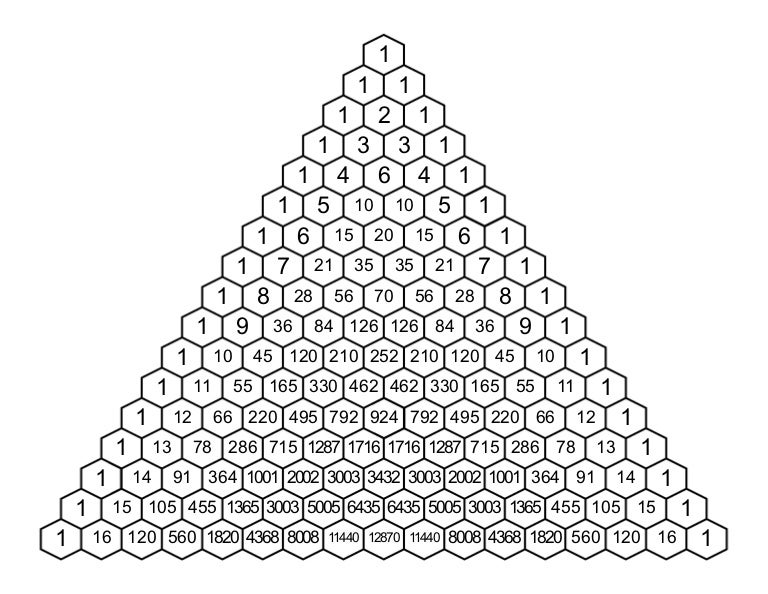
\includegraphics[height=200px]{media/pascal-triangle.jpeg}
   % \caption{Pascal's Triangle}
   % \label{fig:pascal-triangle}
% \end{figure}

\subsection{N-th first terms of P-th column in Pascal Triangle}

\begin{equation}
    \binom{p}{p} + \binom{p+1}{p} + ... + \binom{p+n}{p} = \binom{p+n+1}{p+1}
\end{equation}

\subsection{Number of odd numbers in the N-th line of pascal triangle}

There is a mathematical relation which gives the number of odd numbers in the N-th row of pascal's triangle. The theorem states that the number of odd numbers in N-th row is equal to 2 raised to the number of ones in the binary representation of N.

